
\section{Présentation des données}
%%%%%%%%%%%%%%%%%%%%%%%%%%%%%%%%%%%%%%%%%%%%%%%%%%%%%%%%%%%%%%%%%%%%%%%
\subsection{Présentation}

\subsection{Observation graphique}

\subsubsection{Scatter plot}

\subsubsection{Rank-rank plot}

\subsection{Corrélation de Pearson :  pas une mesure d’association !}

\subsection{Rho de Spearman}

\subsection{Tau de Kendall}

\section{Méthode non paramétrique d'estimation : la copule empirique}
%%%%%%%%%%%%%%%%%%%%%%%%%%%%%%%%%%%%%%%%%%%%%%%%%%%%%%%%%%%%%%%%%%%%%%%
\subsection{Choix d'une copule théorique}


\section{Méthode paramétriques d'estimation}
%%%%%%%%%%%%%%%%%%%%%%%%%%%%%%%%%%%%%%%%%%%%%%%%%%%%%%%%%%%%%%%%%%%%%%%

\subsection{Méthode du maximum de vraisemblance}

\subsection{Méthode IFM (Inference Function for Margins)}


\section{Méthode semi-paramétrique d'estimation (CML)}
%%%%%%%%%%%%%%%%%%%%%%%%%%%%%%%%%%%%%%%%%%%%%%%%%%%%%%%%%%%%%%%%%%%%%%%

Dans cette section, nous allons utiliser la méthode CML (méthode semi-paramétrique) afin d'estimer le paramètre des différentes copules retenues pour modéliser la dépendance entre les données sur Saint-Martin et celles sur Echirolles.
En effet, à l'aide de cette méthode, on peut obtenir une estimation du paramètre de la copule sans se soucier des marginales. Pour cela, il suffit d'utiliser la fonction \textit{fitcopula} de R en passant comme arguments les rangs sur nos deux groupes de données translatés sur $[0;1]$ et un point de départ de l'algorithme. Ce point de départ sera l'estimation du paramètre de la copule obtenue par la méthode des moments. Avec l'estimation du paramètre obtenue en sortie de notre algorithme, on peut alors créer notre copule estimée.

\subsection{Copule de Clayton}

Dans le cas de la copule de Clayton, on obtient, en sortie de l'algorithme, $0,6890$ comme estimation du paramètre de la copule. On peut ainsi tracer les Khi-plot et K-plot de cette copule de Clayton estimé et comparer les graphes avec ceux obtenus pour la copule empirique.

\noindent%
\begin{figure}[H]
    \begin{center}
      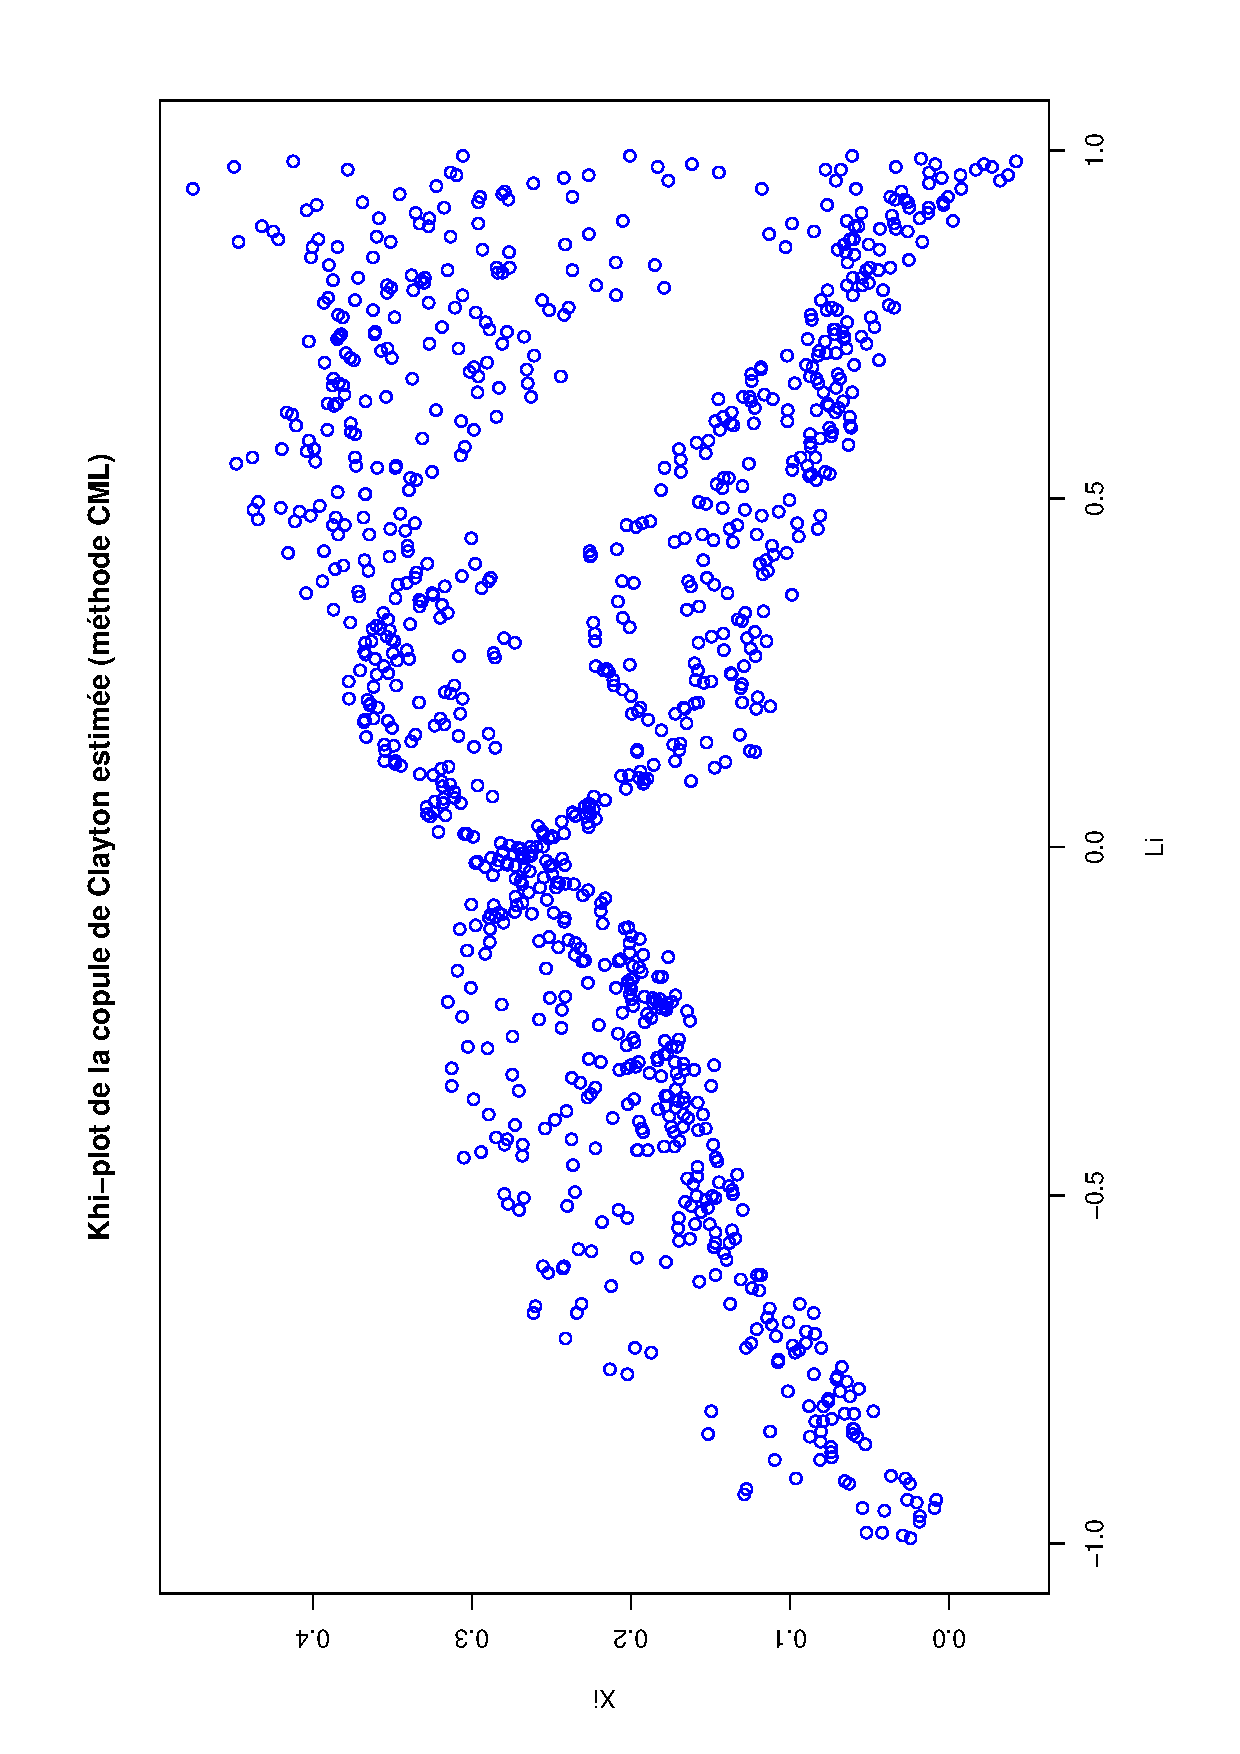
\includegraphics[width=17 cm, angle=0]{./pictures/claytoncmlkhiplot.png}
      \centering\caption{\label{2}Khi-plot de la copule de Clayton estimée (méthode CML)}
    \end{center}
\end{figure}

En comparant ce graphe du Khi-plot avec celui obtenu pour la copule empirique, on peut apercevoir une ressemblance, notamment dûe au fait que les points se répartissent du même côté de l'axe des ordonées (du côté positif) exprimant ainsi une dépendance positive. Cependant, du côté positif de l'axe des abscisses, le nuage de point semble se séparer en deux. Ceci n'est pas observée sur le khi-plot de la copule empirique. 

\noindent%
\begin{figure}[H]
    \begin{center}
      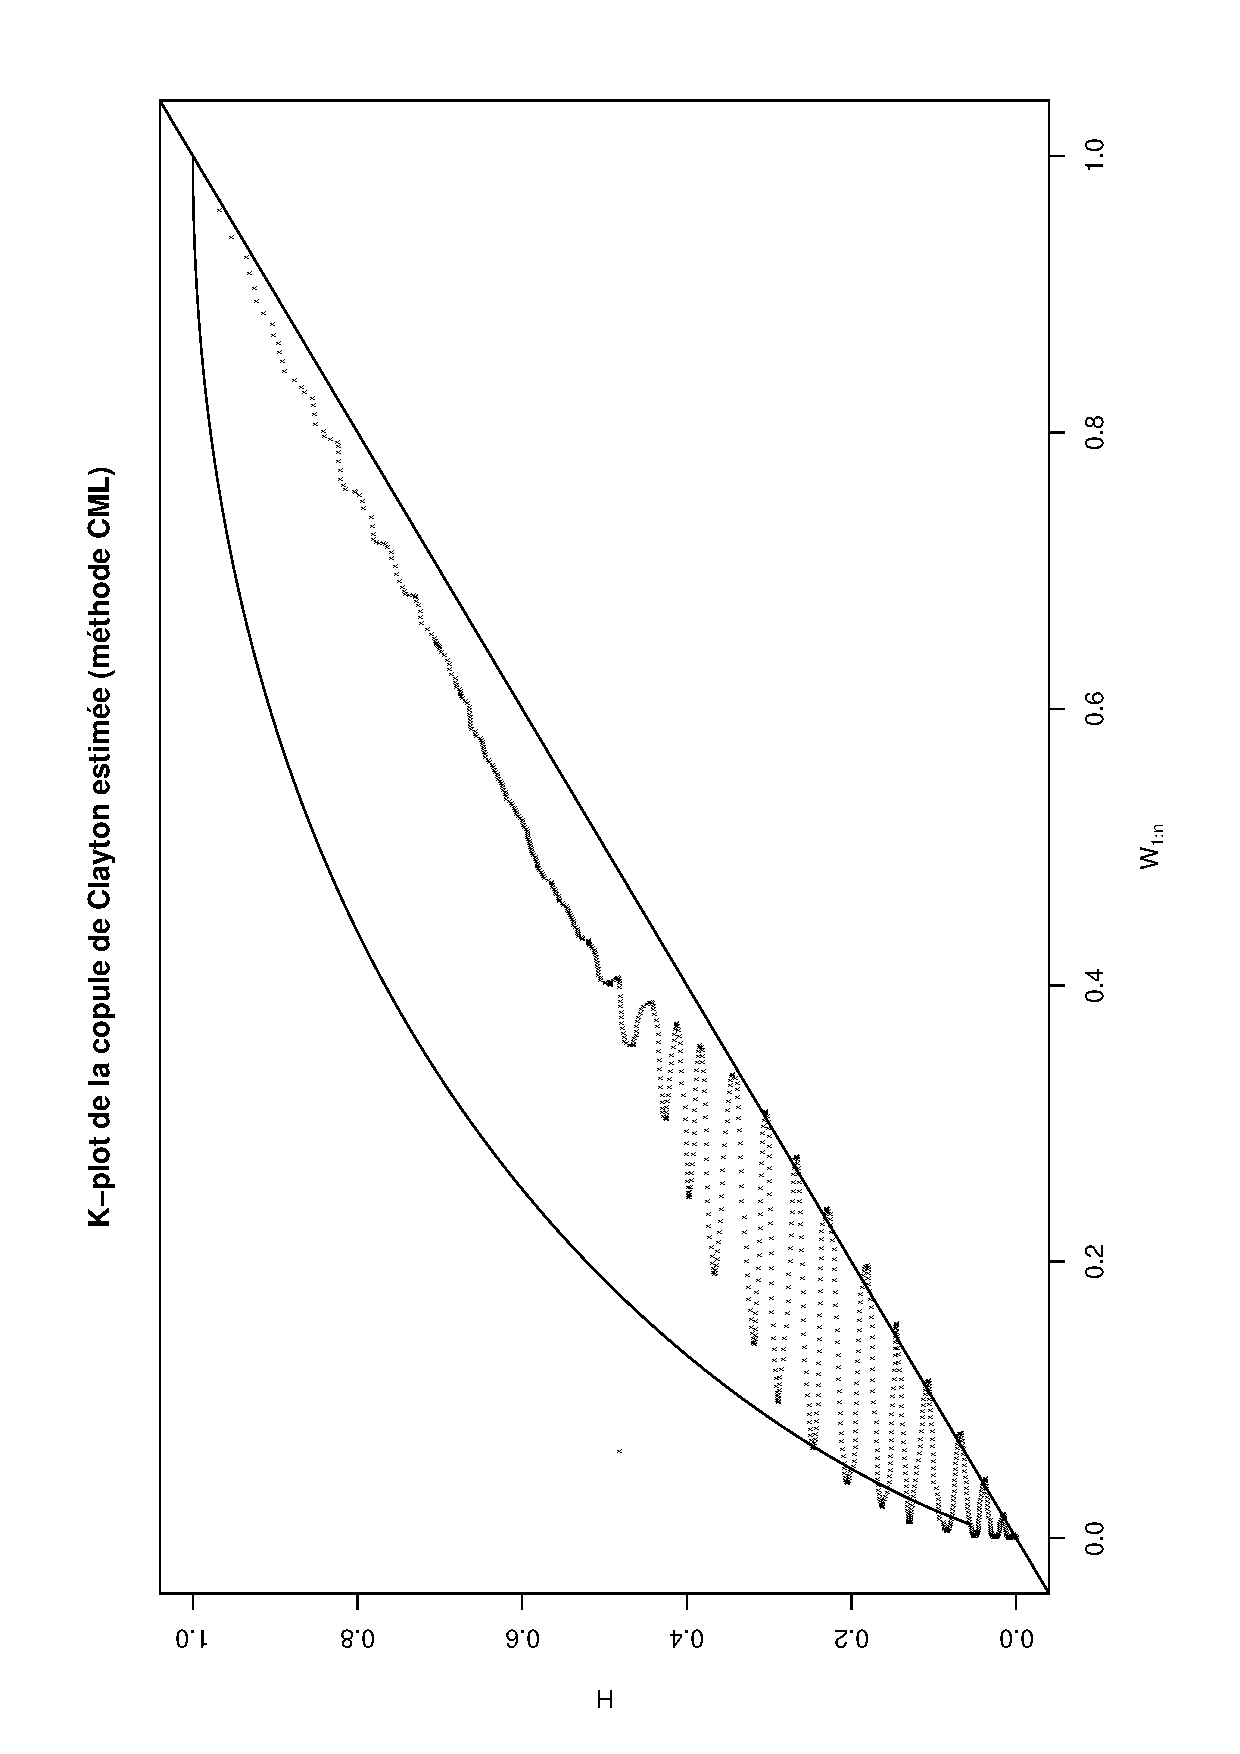
\includegraphics[width=17 cm, angle=0]{./pictures/claytoncmlkplot.png}
      \centering\caption{\label{2}K-plot de la copule de Clayton estimée (méthode CML)}
    \end{center}
\end{figure}

De la même manière, pour ce graphe du K-plot, on observe une similitude et plusieurs disparités par rapport à celui de la copule empirique. En effet, les points semblent se répartir dans le même espace pour les deux figures (globalement entre la courbe de dépendance positive parfaite et la droite d'indépendance $y=x$). Cela montre une nouvelle fois la dépendance positive entre nos deux séries de données. Cependant, concernant le graphe associé à la copule de Clayton estimée, les variations de la répartition des points sont plus grandes et plus nombreuses. Certains points dépassent en effet la courbe de dépendance positive parfaite et on compte également $14$ oscillations distinctes contre $12$ pour le K-plot de la copule empirique. De plus, pour les dernières espérances de statistique d'ordre, les points se rapprochent de la droite $y=x$ alors qu'ils sont proches de la courbe de dépendance positive parfaite pour le graphe concernant la copule empirique.

Ces graphes du Khi-plot et K-plot sont donc d'une certaine façon assez éloignés de ceux obtenus pour la copule empirique.

Pour prolonger nos résultats, on réalise également un algorithme de bootstrap paramétrique. Il s'agit de tester l'adéquation à notre modèle de copule. L'hypothèse nulle du test est donc la suivante:
$$
H_0 : C \in (C_{\theta})
$$
Avec $C_{\theta}$ la famille des copules de Clayton dans notre cas. 
En utilisant les mêmes notations que dans le cours, on rejette l'hypothèse nulle si $D_n > L$. 
Dans notre situation, on obtient, avec un seuil de $0,05$, $D_n = 0,1422 > 0,0463 = L$. De plus, la p-value pour cette statistique de Cramer-Von Mises vaut $0$. La copule empirique ne fait donc pas partie de la famille des copules de Clayton.

En conclusion de cette étude sur la copule de Clayton estimée, on peut considérer que la modélisation de la dépendance entre nos deux séries de données par une copule de Clayton n'est pas satisfaisante.

\subsection{Copule de Gumbel}

\subsection{Copule de Franck}

\subsection{Copule normale}

\subsection{Copule de Student}

\section{Méthode des moments : inversion du tau de Kendall}
%%%%%%%%%%%%%%%%%%%%%%%%%%%%%%%%%%%%%%%%%%%%%%%%%%%%%%%%%%%%%%%%%%%%%%%

Dans cette partie, nous utiliserons la méthode des moments pour estimer le paramètre des copules retenues afin de modéliser la dépendance entre les données sur Saint-Martin et celles sur Echirolles.

\subsection{Copule de Clayton}

\subsection{Copule de Gumbel}

\subsection{Copule de Franck}

\subsection{Copule normale}

\subsection{Copule de Student}

\section{Test graphique d'adéquation à la copule : le Kendall plot}
%%%%%%%%%%%%%%%%%%%%%%%%%%%%%%%%%%%%%%%%%%%%%%%%%%%%%%%%%%%%%%%%%%%%%%%

\subsection{Dépendogramme empirique et dépendogramme théorique}

\subsection{K-plot}

\section{Test statistique d'adéquation à la copule : le Kendall plot}
%%%%%%%%%%%%%%%%%%%%%%%%%%%%%%%%%%%%%%%%%%%%%%%%%%%%%%%%%%%%%%%%%%%%%%%

\subsection{Test de Kolmogorov-Smirnov}

\subsection{La statistique de Cramér-von Mises}

\subsection{Estimation du seuil critique par bootstrap paramétrique}





TODO   TODO   TODO   TODO



%% \noindent%
%% \begin{figure}[H]
%%     \begin{center}
%%       \includegraphics[width=17 cm, angle=0]{./pictures/logchrono1.png}
%%       \centering\caption{\label{2}Logarithme du total des importations de gaz naturel}
%%     \end{center}
%% \end{figure}



